% poster template

\documentclass[20pt,margin=1in,innermargin=-4.5in,blockverticalspace=-0.25in]{tikzposter}
\geometry{paperwidth=42in,paperheight=32.5in}
\usepackage[utf8]{inputenc}
\usepackage{amsmath}
\usepackage{amsfonts}
\usepackage{amsthm}
\usepackage{amssymb}
\usepackage{mathrsfs}
\usepackage{graphicx}
\usepackage{adjustbox}
\usepackage{enumitem}
\usepackage[backend=biber,style=numeric]{biblatex}
\usepackage{uomtheme}

\usepackage{mwe} % for placeholder images

\addbibresource{refs.bib}

% set theme parameters
\tikzposterlatexaffectionproofoff
\usetheme{UoMTheme}
\usecolorstyle{UoMStyle}

\usepackage[scaled]{helvet}
\renewcommand\familydefault{\sfdefault} 
\usepackage[T1]{fontenc}


\title{Algorithm Visualizer: Sorting \& Pathfinding}
\newcommand{\subject}{IT5052, Internet of Things, CIE-3}
\author{Name(Enrollment No), Name(Enrollment No)}
\institute{AMTICS, Uka Tarsadia University}
\titlegraphic{
\includegraphics[width=0.06\textwidth]{UTU.png}}

% begin document
\begin{document}
\maketitle
\centering
\begin{columns}
    \column{0.32}
    \block{Abstract}{
         Monitoring kernel-level activities is vital for system debugging and security auditing. In this project, we expand the capabilities of the xv6-RISC-V operating system by implementing a new \texttt{trace} system call \cite{cite:0}. This feature enables developers to intercept and log system calls executed by a specific process. By utilizing bitmask control \cite{cite:1}, the tracing mechanism is highly selective, logging only the designated system calls along with their return values, thereby providing extensive visibility into the runtime behavior of user-mode programs.
    }
    \block{Introduction}{
         User programs operate in an unprivileged execution mode and rely on specialized \texttt{ecall} hardware instructions to request kernel services like file I/O or process creation \cite{cite:2}. Because these system calls form the boundary between user space and the kernel, observing them is an essential technique for understanding application behavior.
         
         The primary objective of this project is to implement a per-process system call interception layer. A significant challenge in this environment is enforcing process isolation so that activating tracing on one process does not inadvertently impact others. The newly introduced \texttt{trace} system call seamlessly hooks into the central system call switchboard, filtering and logging relevant calls automatically based on a user-defined mask.
    }
    \block{System Implementation}{
        We implemented the tracing feature through several modifications to the xv6 kernel architecture:
        
        \begin{itemize}
            \item \textbf{Process Structure (\texttt{proc.h})}: We extended the Process Control Block (\texttt{struct proc}) to include an integer \texttt{trace\_mask}, ensuring that tracing configurations remain completely isolated between different processes.
            \item \textbf{Configuration (\texttt{sysproc.c})}: We added \texttt{sys\_trace()}, a function that retrieves the bitmask argument from the user's trapframe using the \texttt{argint()} helper, and stores it in the current process's \texttt{trace\_mask}.
            \item \textbf{Inheritance (\texttt{proc.c})}: During process duplication (\texttt{fork()}), the parent's \texttt{trace\_mask} is copied to the child process. This allows the tracing to persist when a command-line utility executes new programs via \texttt{exec()}.
        \end{itemize}
    }

    \column{0.36}
    \block{Features \& Logic}{
        At the core of the implementation is the centralized \textbf{Dispatch Execution Logic} within \texttt{syscall.c}. Instead of modifying the implementation of every individual system call, we intercepted the generic \texttt{syscall()} dispatch function. 
        
        The execution relies on bitwise operations to check permissions before printing:
        \vspace{0.5em}
        \begin{itemize}
            \item The argument is interpreted as a \textbf{bitmask}. For instance, tracing only \texttt{SYS\_read} (which has the syscall number 5) uses the mask $32$ ($1 \ll 5$).
            \item After the designated system call finishes executing, the kernel tests the exact bit: \\ \texttt{if(p->trace\_mask \& (1 $\ll$ num))}
            \item If the operation yields a non-zero value, the kernel outputs a formatted message containing the PID, the human-readable syscall name, and the syscall's return value.
        \end{itemize}
        \vspace{1em}
        \begin{tikzfigure}[Syscall Tracing Flow architecture.]
            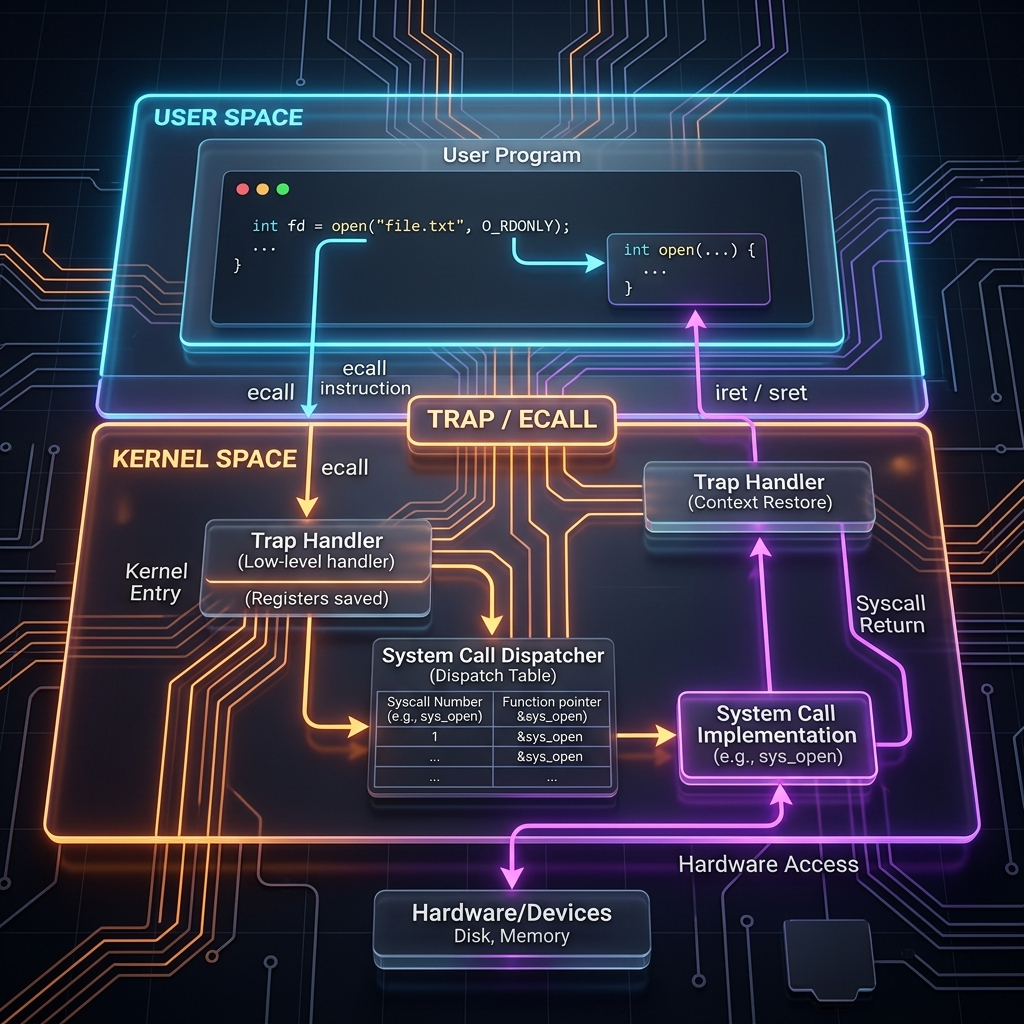
\includegraphics[width=0.9\linewidth]{poster_hero_image.png}
        \end{tikzfigure}
        \vspace{1em}
        Furthermore, we integrated a \texttt{syscall\_names} array to dynamically map raw system call integers to human-readable string values during the print sequence, drastically enhancing the usability of the resulting trace logs.
    }

    \column{0.32}
    \block{Results \& Metrics}{
        The completed project provides real-time audit logs of system execution with zero overhead for untraced processes. A user can trace operations smoothly using the newly added command-line program \cite{cite:3}:
        
        \textbf{Usage Example:} \texttt{trace 32 grep hello README}
        
        \textbf{Output:} 
        The system precisely isolates read commands in the terminal feed:
        \begin{itemize}
            \item \texttt{3: syscall read -> 1023}
            \item \texttt{3: syscall read ->   966}
            \item \texttt{3: syscall read ->     0}
        \end{itemize}
        
        \begin{tikzfigure}[Sample trace log execution.]
            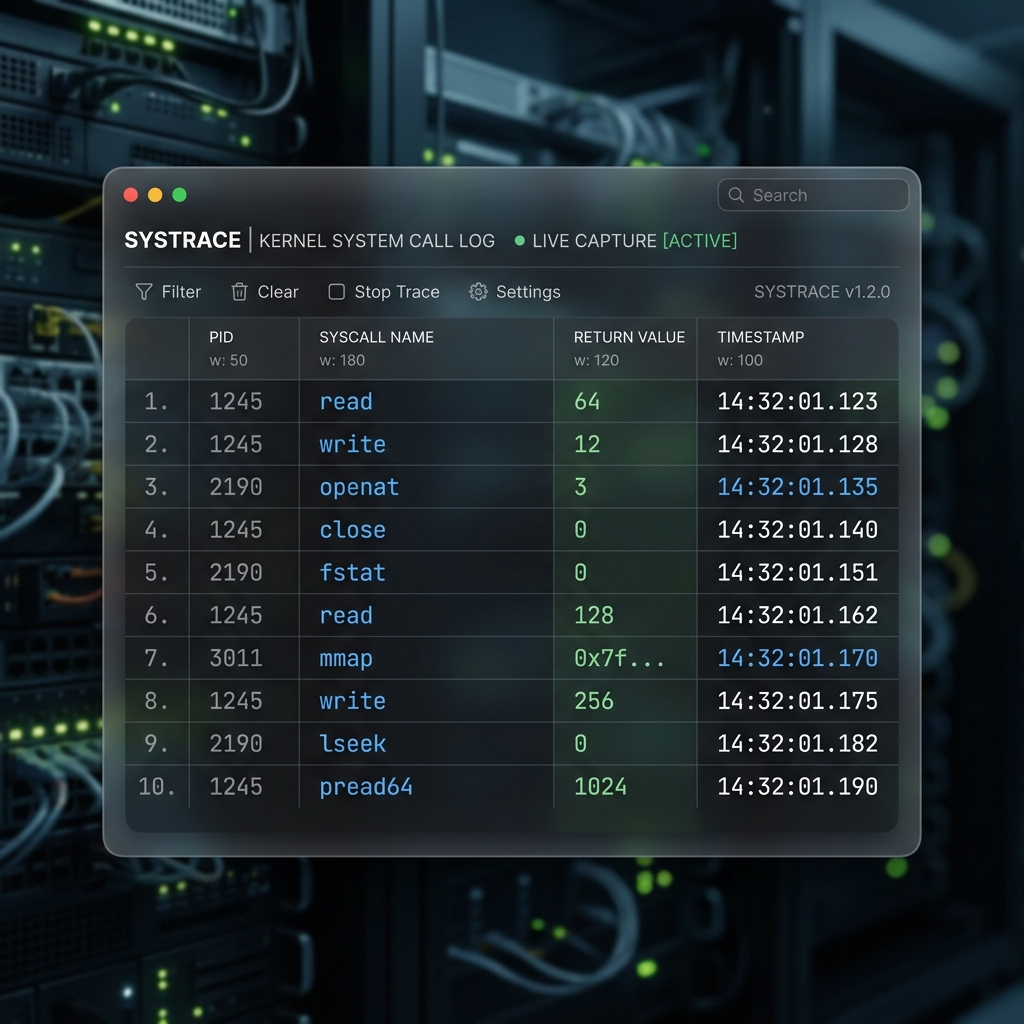
\includegraphics[width=0.5\linewidth]{metrics_panel.png}
        \end{tikzfigure}
    }
    
    \block{Conclusion}{
        Through this work, we effectively expanded the xv6 process structures to securely intercept and log kernel tasks via the \texttt{trace} system call. By storing the configuration within each \texttt{struct proc} and integrating directly into the primary \texttt{ecall} trap handler, we maintained robust process isolation while bridging the transparency gap between user executables and kernel functions.
    }
    
    \block{Future Scope}{
        In the future, the tracing framework could be extended to allow the extraction and formatting of dynamic parameter types passed into system calls (e.g., string arguments for \texttt{open} or memory addresses for \texttt{sbrk}). We also intend to explore saving trace output directly to a persistent file to support the logging of massive applications.
    }
    
    \block{References}{
        \vspace{-1em}
        \begin{footnotesize}
        \printbibliography[heading=none]
        \end{footnotesize}
    }
\end{columns}
\end{document}